\subsection{Beta Value:}

To measure the $\beta$ value using a multimeter or any other device that has the option {\bfseries\itshape hfe} it's very simply, once the multimeter it's on this option the only thing you need to do it's search on the device the following section:

\begin{figure}[H]
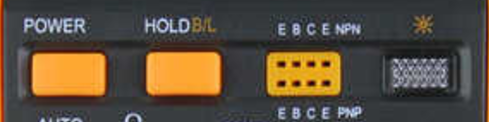
\includegraphics[height = 2cm, width = 10cm]{p0.png}
\centering \linebreak \linebreak Figure 3.1.0: Multimeter NPN - PNP section.
\end{figure}

As we can see in Figure 3.1.0, there are at least 8 little holes, on the top we can see the label {\bfseries\itshape NPN} and {\bfseries\itshape PNP} on the bottom, and beside this two labels we have {\bfseries\itshape E - B - C - E}. As you can imagine this are shortenings for {\bfseries\itshape emitter - collector - base}. So, in case you put the terminals of the transistor in this holes, you can figure it out which terminal belongs to the emitter, the base and the collector. \hfill \break

Once we measure the $\beta$ for the transistors {\bfseries\itshape 2N2222A, BC547C} and {\bfseries\itshape BC557C}, the results were captured in the following table: \hfill \break

\begin{center}
\begin{tabular}[5cm]{c c c c}
\toprule
\toprule
\hspace{80pt} & \hspace{35pt} 2N2222A \hspace{35pt} & \hspace{35pt} BC547C \hspace{35pt} & \hspace{35pt} BC557C \hspace{35pt} \\
\midrule
\midrule
$\beta$ & 241 & 595 & 630 \\ 
\bottomrule
\linebreak
\end{tabular}
\linebreak Table 1: Beta values for the development transistors.
\end{center} \hfill \break 

{\bfseries\itshape\color{carmine}{Observation:}} {\itshape\color{carmine}{This values are used as well in the {\bfseries Theoretical analysis} in section 5.}}

\pagebreak